%%%%%%%%%%%%%%%%%%%%%%%%%%%%%%%%%%%%%%%%%%%%%%%%%%%%%%%%%%%%%%%%%%%%%%%%
%                                                                      %
%     File: Implementation/05_SoftwareArchitecture.tex                 %
%     Tex Master: ../Thesis.tex                                        %
%                                                                      %
%%%%%%%%%%%%%%%%%%%%%%%%%%%%%%%%%%%%%%%%%%%%%%%%%%%%%%%%%%%%%%%%%%%%%%%%

% ==============================================================================
\section{Software Architecture and Mission Control}
\label{sec:software_architecture_and_dashboard}

% What does this section present?
The models, controllers and manoeuvres of the previous sections are implemented as independent software components, integrated with the simulator and with the autopilot of the \gls{uav}. This section describes the architecture that connects these components and the interface through which an operator executes the missions. The code of the system is publicly available at \url{https://github.com/tomasgesteves1/tethered-usv-uav-nmpc}.

\subsection{Architecture}
\label{subsec:integrated_software_architecture}

% How is the software organised?
The software is built on \gls{ros}~2~\cite{macenski2022ros2}, in which each component runs as an independent node, and the nodes exchange messages through named topics. The controllers therefore do not depend on whether their data comes from the simulation or from the real vehicles.

% How are the components connected?
Figure~\ref{fig:architecture} shows the components and the main data exchanged between them. Gazebo simulates the vehicles and the waves, while PX4 runs as the autopilot of the \gls{uav}, in lockstep with the simulation. Each is connected to \gls{ros}~2 by a bridge, the ROS--Gazebo bridge~\cite{ros_gz} and the Micro XRCE-DDS agent~\cite{micro_xrce_dds}. The tether node applies in Gazebo the force of the tether, computed by MoorDyn~\cite{hall2015moordyn} for the length set by the winch. The two \gls{nmpc} controllers send their commands to the thrusters of the \gls{usv} and to the autopilot of the \gls{uav} while exchanging their predicted trajectories, and the mission executor produces the references of both. A web server connects \gls{ros}~2 to a Mission Control Centre.

\begin{figure}[htbp]
    \centering
    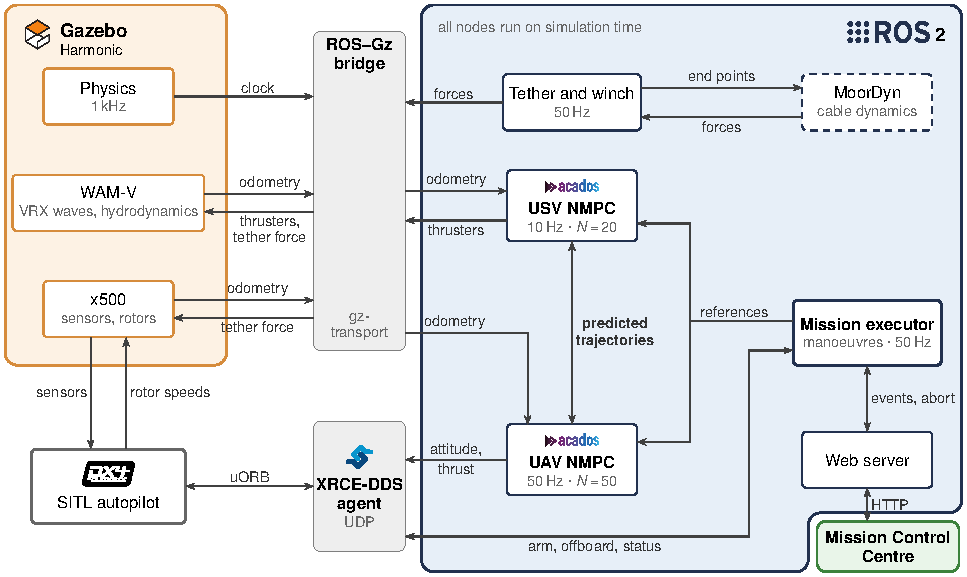
\includegraphics[width=0.85\textwidth]{Implementation/figures/05_software_architecture/architecture.pdf}
    \caption{Software architecture.}
    \label{fig:architecture}
\end{figure}

\subsection{Mission Control Centre}
\label{subsec:operator_dashboard}

% What is the Mission Control Centre for?
The Mission Control Centre is a web page, shown in Figure~\ref{fig:mission_control_centre}, from which an operator runs the whole system without the command line. Since every mission is launched and recorded in the same way, it also made the tests in simulation repeatable. It is organised in four parts.
\begin{itemize}
    \item \textbf{Simulation}, at the top, starts and stops the simulation, with or without the graphical interface of Gazebo.
    \item \textbf{Missions}, on the left, lists the missions with their manoeuvres, starts one, optionally recording its data, and aborts it.
    \item \textbf{Map}, in the centre, shows the two vehicles, the tether and their references from above.
    \item \textbf{Telemetry and progress}, on the right, show the state of each vehicle and of the tether, and the manoeuvres of each vehicle already done, running and still to come.
\end{itemize}

\begin{figure}[H]
    \centering
    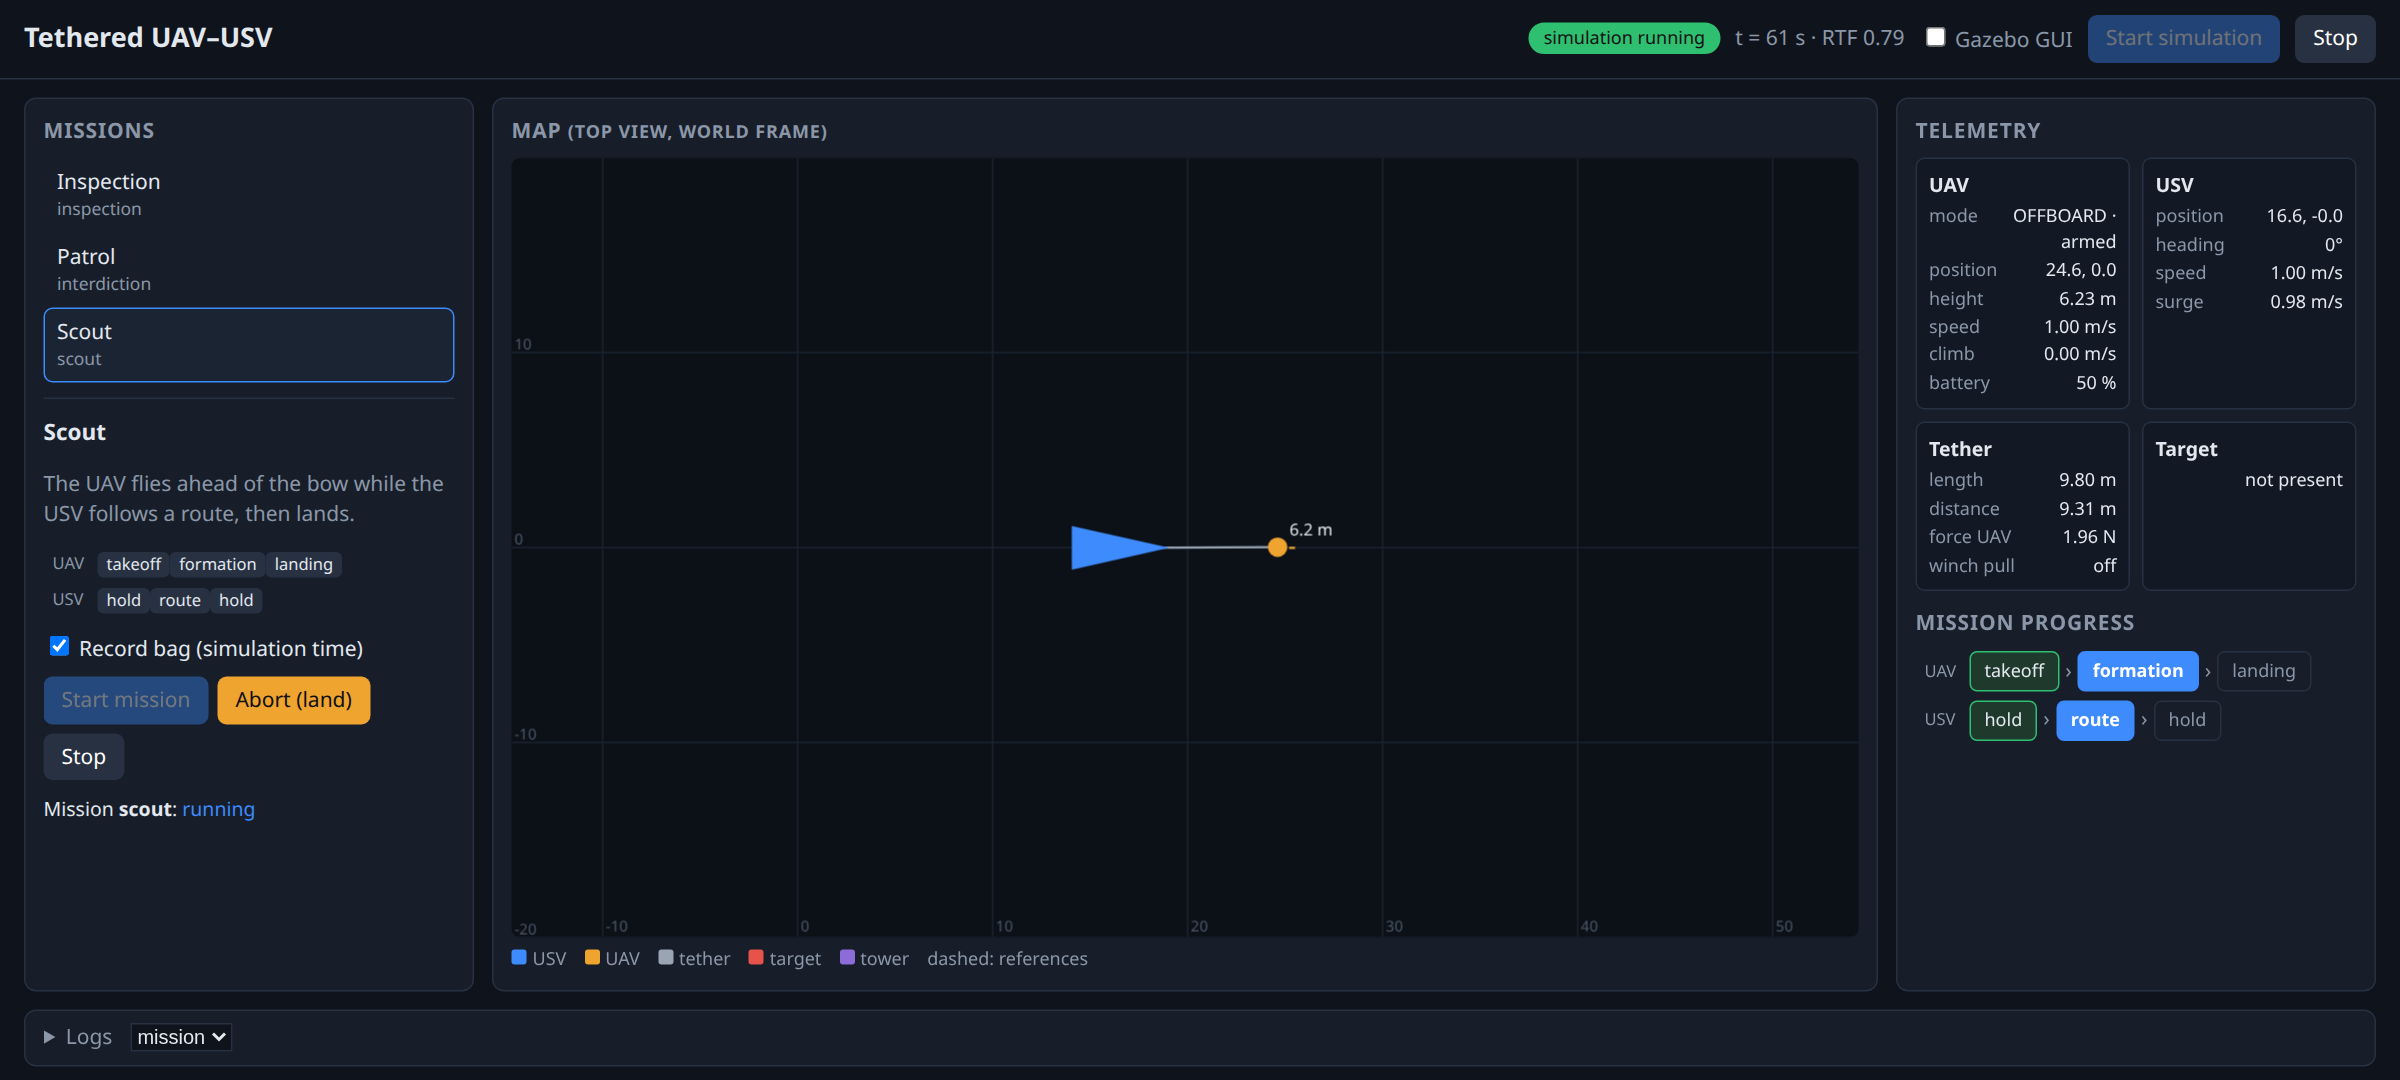
\includegraphics[width=1.0\textwidth]{Implementation/figures/05_software_architecture/mission_control_centre.png}
    \caption{Mission Control Centre during the scout mission.}
    \label{fig:mission_control_centre}
\end{figure}
